\documentclass[conference]{IEEEtran}

% Packages
\usepackage{graphicx}
\usepackage{amsmath}
\usepackage{url}
\usepackage{hyperref}
\usepackage{balance} % To balance columns on the last page
\usepackage{amsfonts, amssymb} % Added for more math symbols, from IEEE template
\usepackage{subfig} % Added to support subfigures (Fig 7a, 7b, 7c)


% Correct bad hyphenation
\hyphenation{op-tical net-works semi-conduc-tor intel-li-gi-bil-i-ty spec-tro-gram Lev-en-shtein}

\begin{document}

% Paper title
\title{Exploratory Data Analysis for Lyric Intelligibility Prediction:\\
ICASSP 2026 Cadenza CLIP1 Challenge}

% Author information
\author{
    \IEEEauthorblockN{Muhammad Musaab Ul Haq (501739)}
    \IEEEauthorblockA{\textit{SEECS, NUST} \\
    Islamabad, Pakistan}
    \and
    \IEEEauthorblockN{Usman Amjad (516261)}
    \IEEEauthorblockA{\textit{SEECS, NUST} \\
    Lahore, Pakistan}
    \and
    \IEEEauthorblockN{Ahmed Hassan Raza (511263)}
    \IEEEauthorblockA{\textit{SEECS, NUST} \\
    Lahore, Pakistan}
    \and
    \IEEEauthorblockN{Abdul Mueed Habib Raja (501166)}
    \IEEEauthorblockA{\textit{SEECS, NUST} \\
    Chasma, Pakistan}
}


% Make the title area
\maketitle

% Abstract
\begin{abstract}
This report presents an exploratory data analysis (EDA) of the Cadenza CLIP1 dataset. The goal of this challenge is to predict how well people with hearing impairments can understand song lyrics when using different hearing aids. Our analysis looks at four main areas: (1) the general distribution of intelligibility scores, (2) how word-level features affect understanding, (3) the role of audio properties, and (4) how listener mistakes relate to the scores. By exploring the entire training dataset, we engineered features to find what factors influence lyric intelligibility. These findings provide a starting point for building a model to help improve hearing aids for listening to music.
\end{abstract}

% Keywords
\begin{IEEEkeywords}
Hearing aids, lyric intelligibility, audio signal processing, exploratory data analysis, assistive technology.
\end{IEEEkeywords}

% Introduction
\section{Introduction and Motivation}
Listening to music is often difficult for hearing aid users. While modern hearing aids are good at making speech clearer in noisy places, the complicated sounds in music, especially song lyrics, are a major challenge. The ICASSP 2026 Cadenza CLIP1 challenge aims to solve this problem by asking participants to predict how well a person with hearing loss can understand lyrics. The task can be done through two methods. One method would be directly calculate the score through the use of audio and perform operations on the audio and evaluate the score from that. Another approach given to us, is to use the whisper model and convert to text first and then perform an evaluation criteria from the text such that it results in the correction score.

The main objective is to build a model that can predict a listener's understanding of lyrics based on their hearing aid settings. This is important for a few reasons:
\begin{itemize}
    \item It can help create better hearing aids for music.
    \item It allows for personalized settings for each user.
    \item It can improve the quality of life for music lovers with hearing loss.
\end{itemize}

\section{Dataset Overview}
The Cadenza CLIP1 dataset is large and contains thousands of audio clips and corresponding listener data. It gives us everything we need to analyze this problem and includes a few key types of data (modalities):
\begin{itemize}
    \item \textbf{Audio Signals}: Music clips are provided in two versions: the original, unprocessed audio and the version processed by a simulated hearing aid.
    \item \textbf{Listener Transcripts}: Text of what listeners thought they heard.
    \item \textbf{Ground Truth Lyrics}: The actual lyrics from the song.
    \item \textbf{Intelligibility Scores}: A score from 0 to 1 that tells us how much of the lyrics the listener understood correctly.
    \item \textbf{Hearing Profiles}: Information on the type of hearing loss for each listener (e.g., Mild, Moderate).
\end{itemize}
An example entry includes a processed audio file, the listener's attempt at transcribing the lyrics (e.g., "I see a red door"), the true lyric ("I see a red door and I want it painted black"), and a correctness score.

\section{Exploratory Data Analysis (EDA)}

\subsection{Distribution of Intelligibility Scores}
First, we looked at the distribution of the "correctness" scores, which is our target variable. As shown in Figure~\ref{fig:target_dist}, the scores form two main groups. There is a large peak of very high scores (above 0.8) and another large peak of very low scores (below 0.2). This suggests that listeners either understood the lyrics very well or not at all, with fewer people in the middle. This observation is important because it might mean we can classify listeners into "high understanding" and "low understanding" groups. \textbf{For each of the analysis following from here onward, there would be a corelation score at the top right of the plot,  to allow the reader to comprehend the corelation between the two variables in a much more clearer manner (as some plots often have too many scattered points).}

\textit{\textbf{The corelation score is the variable 'r'.
}}
\begin{figure}[htbp]
    \centering
    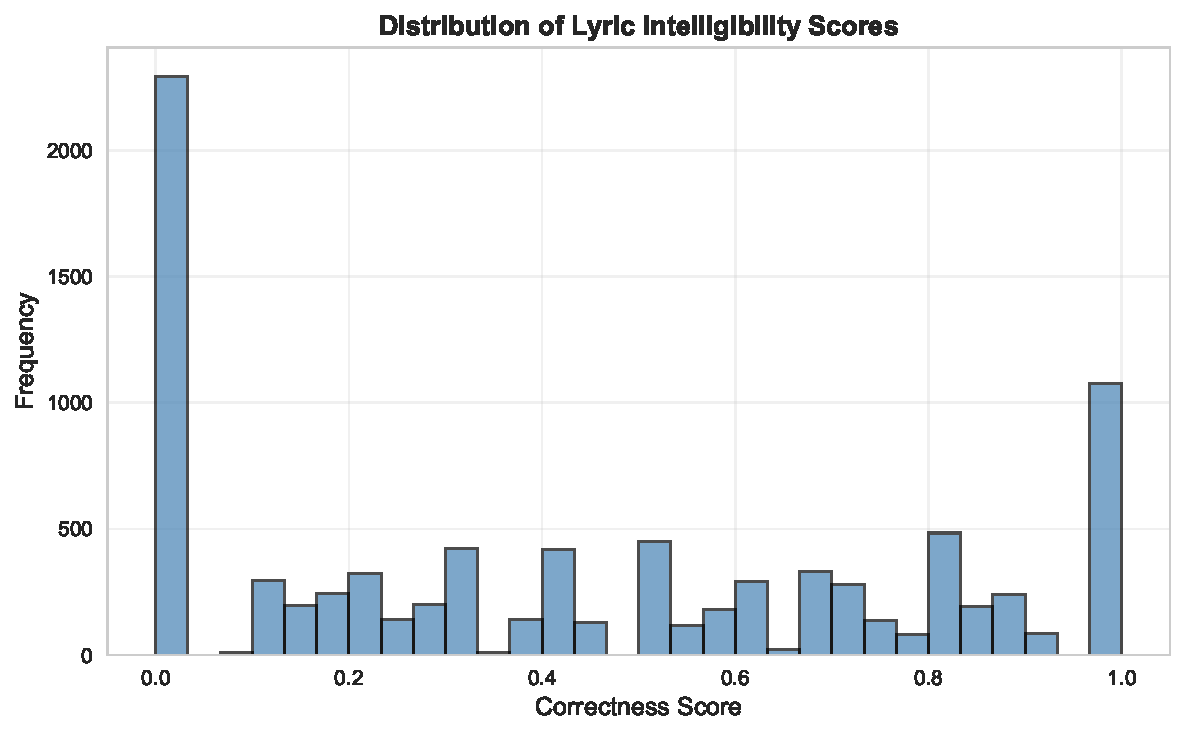
\includegraphics[width=\columnwidth]{plots_assignment_1/figure_1_target_distribution.pdf}
    \caption{Distribution of lyric intelligibility scores, showing two distinct groups of listeners.}
    \label{fig:target_dist}
\end{figure}

\subsection{Signal Comparison}
Figure~\ref{fig:signal_comp} compares an original audio clip with its processed version. The waveforms and spectrograms show that the processing changes the audio's amplitude and frequency content by quite a big difference. It dampens alot of the larger amplitudes.

\begin{figure}[htbp]
    \centering
    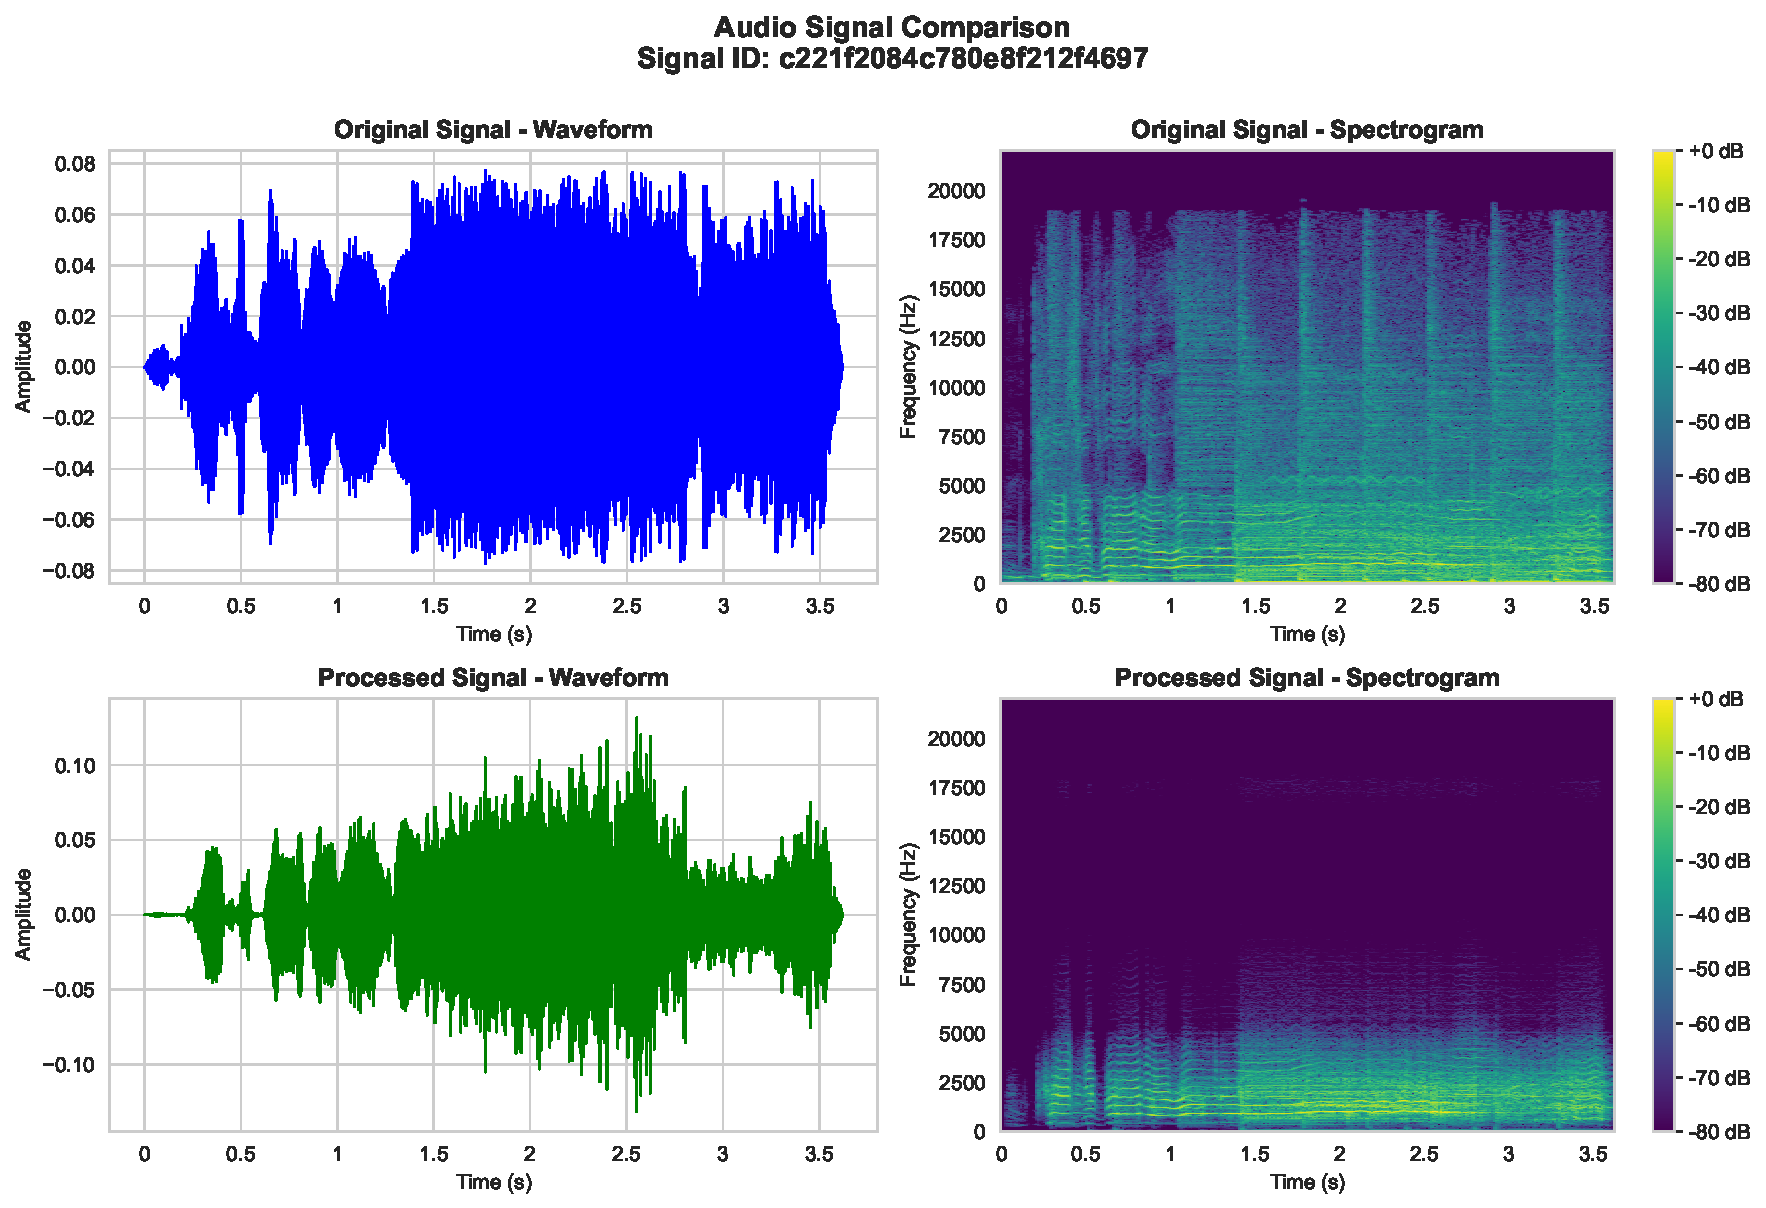
\includegraphics[width=\columnwidth]{plots_assignment_1/figure_2_signal_comparison.pdf}
    \caption{A comparison of original and processed audio signals.}
    \label{fig:signal_comp}
\end{figure}

\subsection{Linguistic Features}
We explored if the words themselves made understanding harder.
\begin{itemize}
    \item \textbf{Word Length}: Figure~\ref{fig:word_length} shows that there is a slight negative trend (albeit small enough to be neglegible, r=-0.098) between the average word length and the intelligibility score. Our hypothesis was that lyrics with longer words might be a bit harder to understand but that seems to be untrue to a large extent.
    \item \textbf{Word Frequency}: We also checked if common words are easier to hear. In Figure~\ref{fig:word_freq}, we see that the hypothesis 'words that are moderately common tend to have the highest intelligibility scores' is hardly true, given the corelation score of only -0.020. 
\end{itemize}

\begin{figure}[htbp]
    \centering
    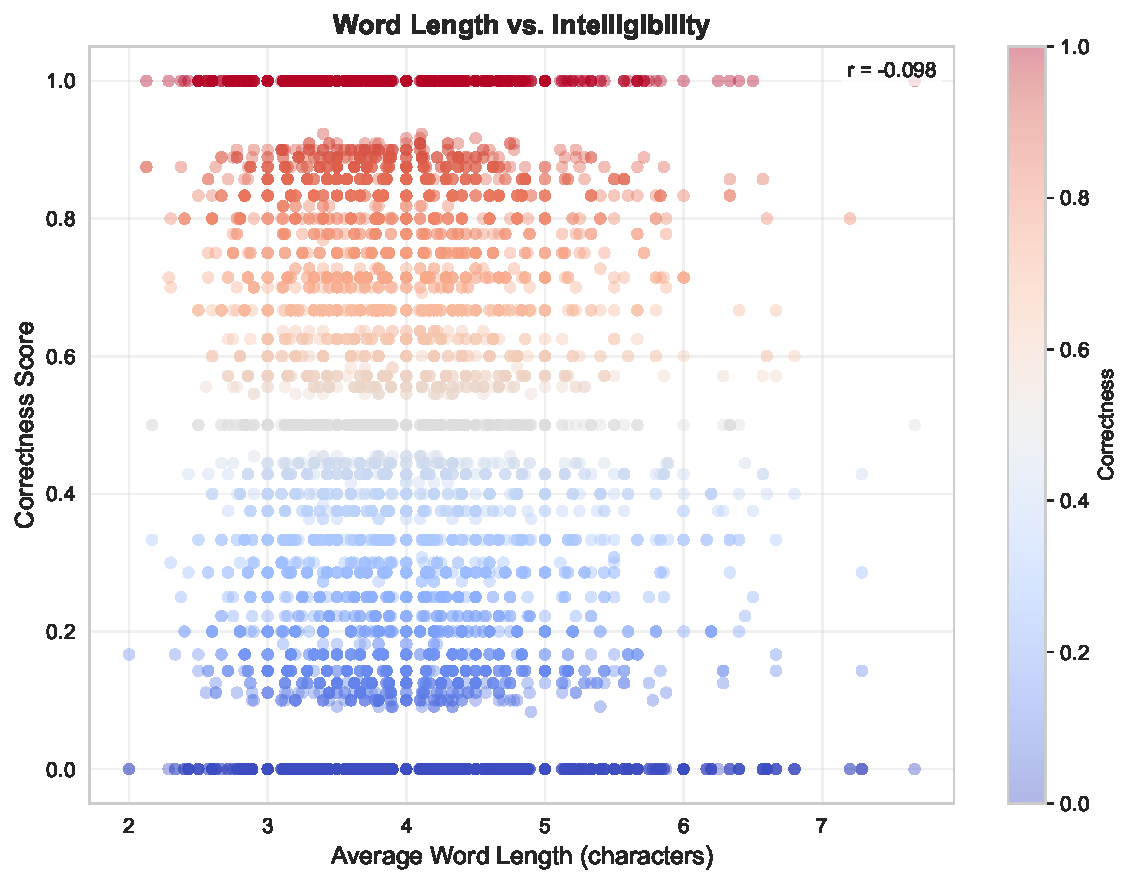
\includegraphics[width=\columnwidth]{plots_assignment_1/figure_3_word_length.pdf}
    \caption{Longer words show a slight trend towards lower intelligibility.}
    \label{fig:word_length}
\end{figure}

\begin{figure}[htbp]
    \centering
    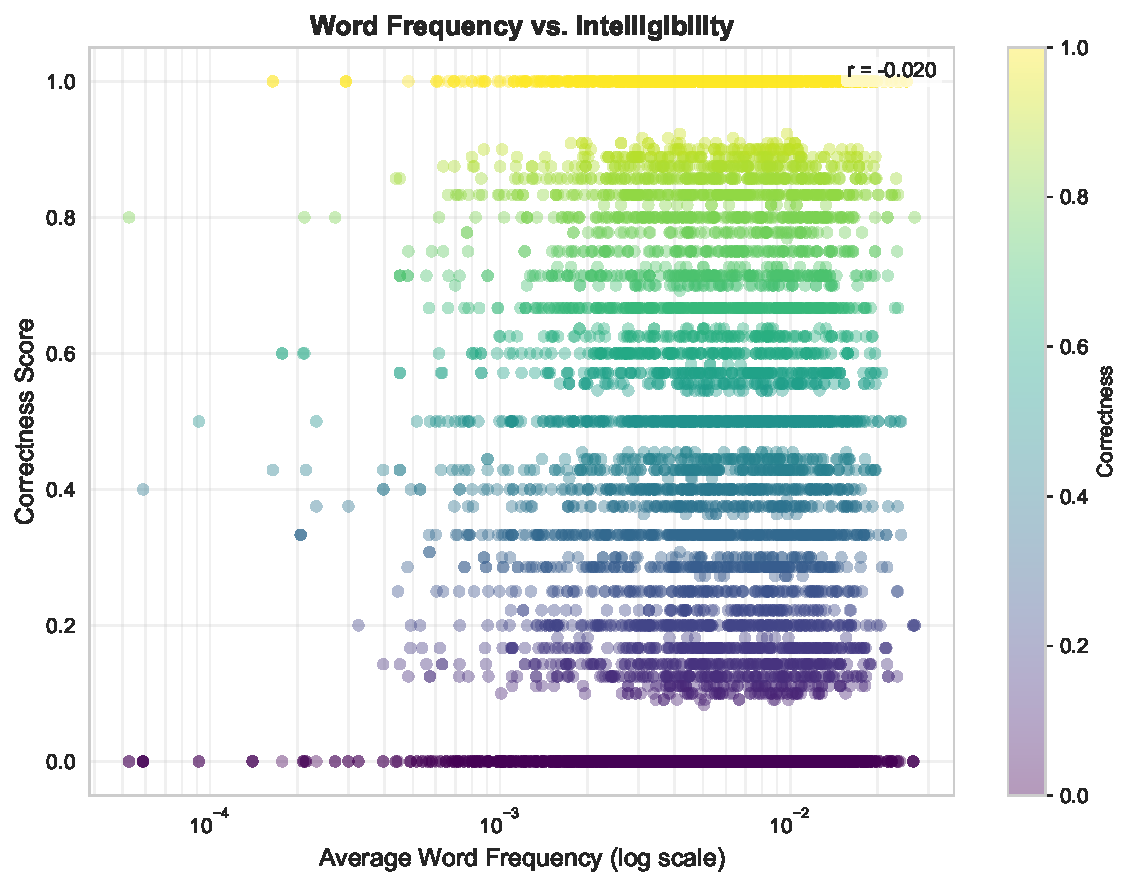
\includegraphics[width=\columnwidth]{plots_assignment_1/figure_4_word_frequency.pdf}
    \caption{Moderately common words appear to be the easiest to understand.}
    \label{fig:word_freq}
\end{figure}

\subsection{Acoustic Analysis}
We analyzed the audio's "brightness" using a feature called the spectral centroid. Figure~\ref{fig:spectral} (figure at next page) shows that intelligibility is somewhat correlated to spectral centroid. This suggests that an optimal frequency range does affect lyric clarity.

\begin{figure}[htbp]
    \centering
    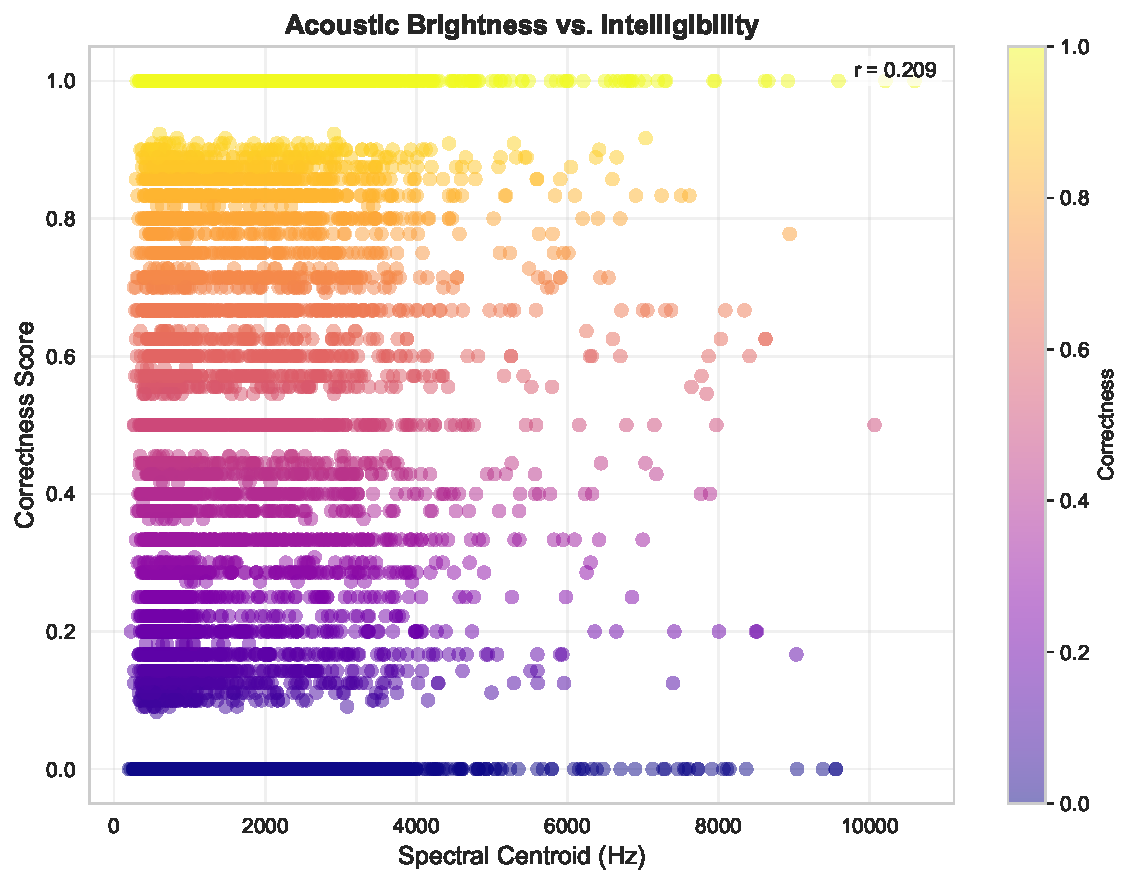
\includegraphics[width=\columnwidth]{plots_assignment_1/figure_5_spectral_centroid.pdf}
    \caption{An optimal "brightness" range seems to exist for the best lyric understanding.}
    \label{fig:spectral}
\end{figure}

\subsection{Listener Error Analysis}
To confirm that the correctness score is a good measure of understanding, we compared it to the number of mistakes in the listeners' transcriptions. We used the normalized Levenshtein edit distance to count these mistakes. Figure~\ref{fig:edit_dist} (figure at next page) shows a strong inverse relationship: as the number of mistakes (edit distance) goes up, the correctness score goes down. This confirms the edit distance can be a reliable metric for identifying correct lyrics. Unfortunately, edit score requires text and cant be directly applied to audio, hence if we would be approaching the task from approach 2, only then can we apply this metric in some form. If confused what I mean by approach 2, then please refer to \textbf{Introduction and Motivation} section.

\begin{figure}[htbp]
    \centering
    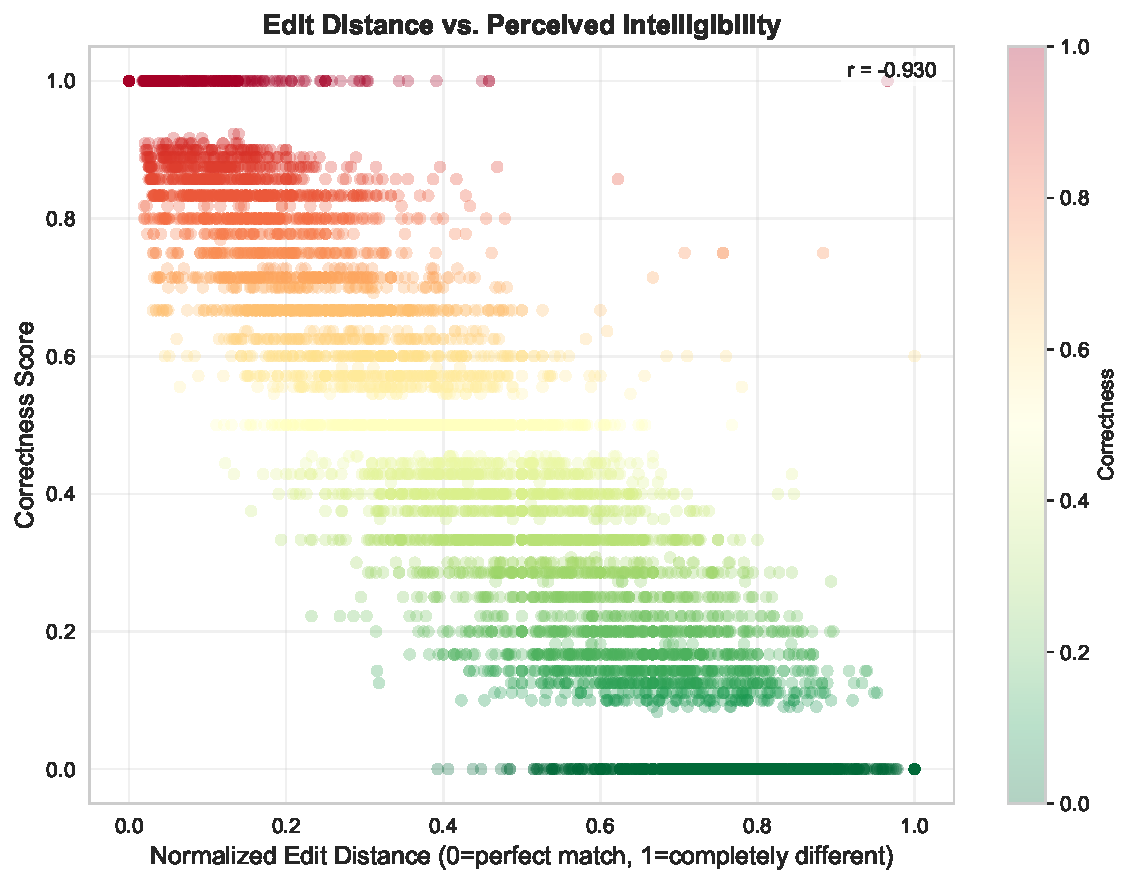
\includegraphics[width=\columnwidth]{plots_assignment_1/figure_6_edit_distance.pdf}
    \caption{Fewer transcription mistakes (lower edit distance) strongly correlates with higher intelligibility scores.}
    \label{fig:edit_dist}
\end{figure}

\subsection{Analysis Across Hearing Loss Groups}
Finally, we wanted to see if these trends were different for people with different levels of hearing loss. Figure~\ref{fig:synthesis}  (figure attached at the end) splits the word length analysis by hearing loss category. It shows that the negative effect of longer words is stronger for listeners with more severe hearing loss, if we find the ratio of corelation among all the loss category. This is a weak insight, as it suggests that the best prediction models will need to take a listener's individual hearing profile into account.

\begin{figure*}[t!]
    \centering
    \subfloat[Mild Hearing Loss]{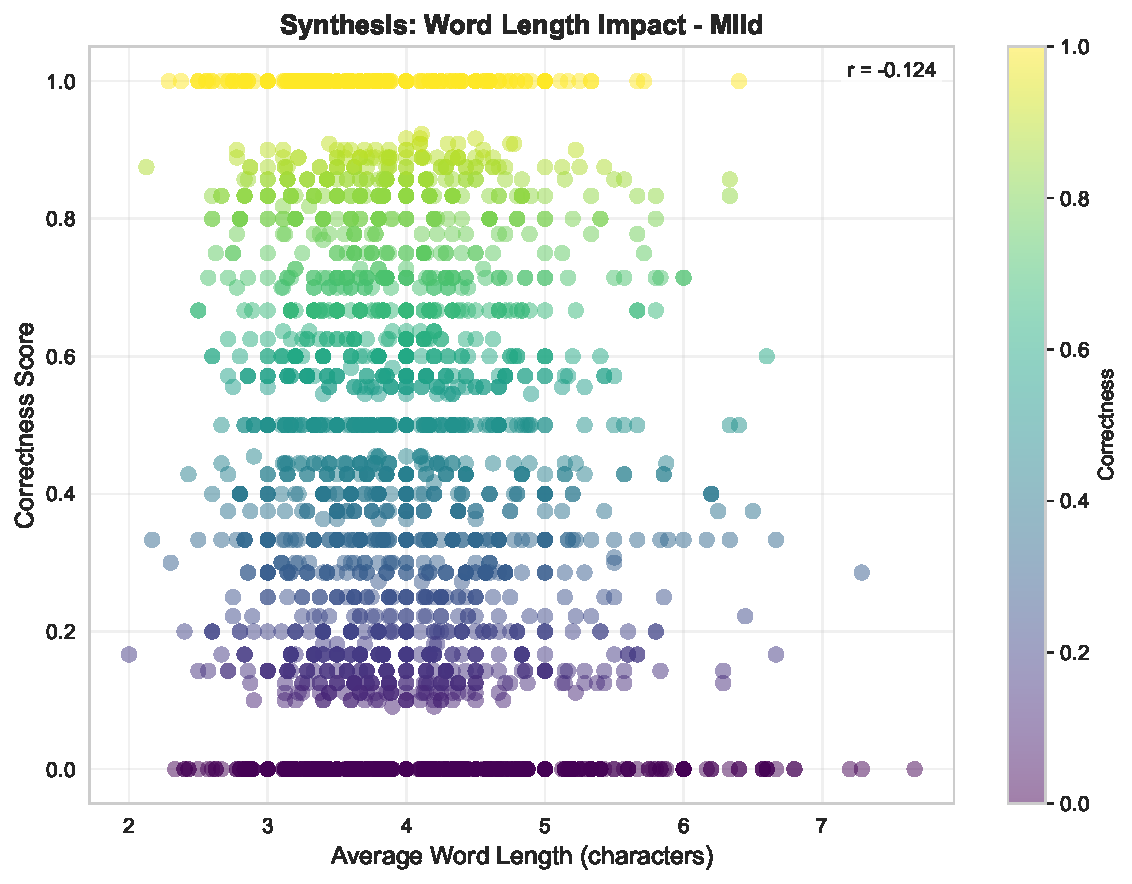
\includegraphics[width=0.32\textwidth]{plots_assignment_1/figure_7a_synthesis_interaction_Mild.pdf}\label{fig:7a}}
    \hfill
    \subfloat[Moderate Hearing Loss]{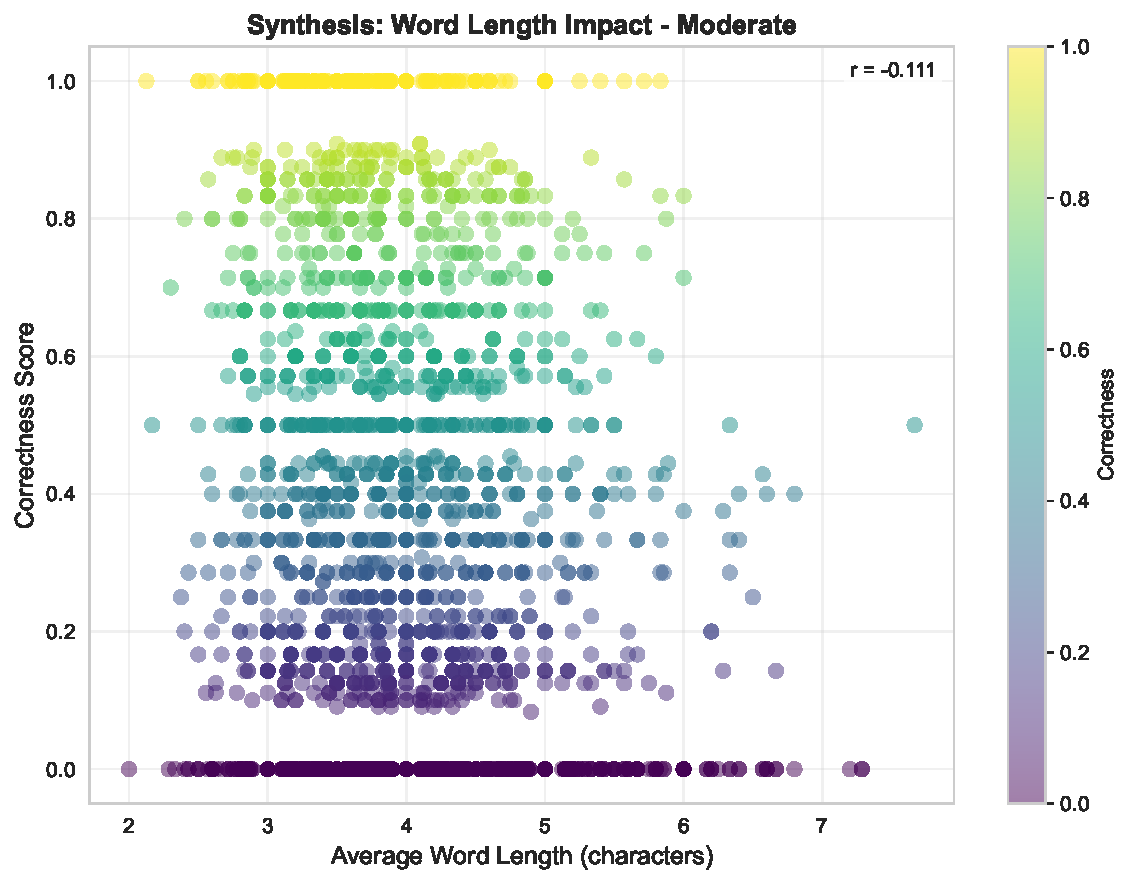
\includegraphics[width=0.32\textwidth]{plots_assignment_1/figure_7b_synthesis_interaction_Moderate.pdf}\label{fig:7b}}
    \hfill
    \subfloat[No Hearing Loss]{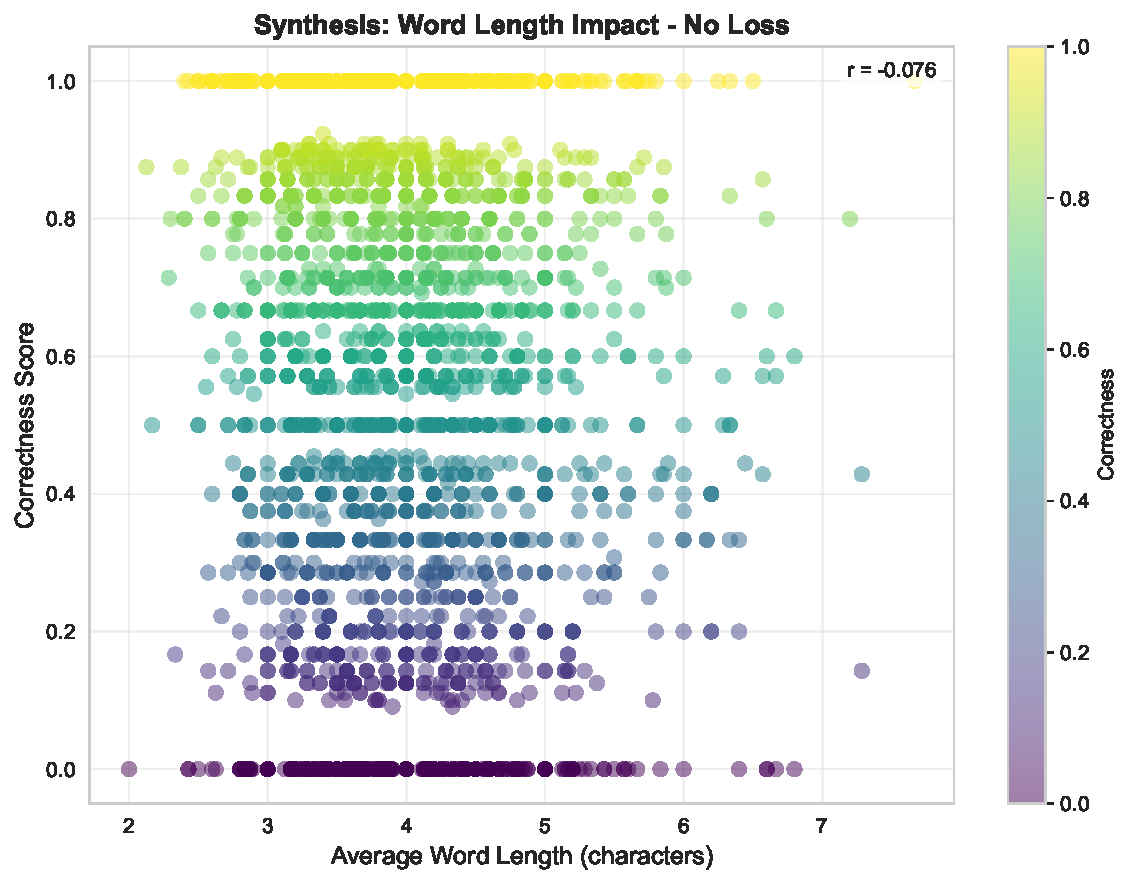
\includegraphics[width=0.32\textwidth]{plots_assignment_1/figure_7c_synthesis_interaction_No Loss.pdf}\label{fig:7c}}
    \caption{The impact of word length on intelligibility for different hearing loss groups. The negative trend is stronger for those with more severe hearing loss.}
    \label{fig:synthesis}
\end{figure*}

\section{Problem Formulation and Metrics}
\subsection{Problem Formulation}
The main task is to predict the lyric intelligibility for a given listener and audio clip. This is a regression problem where the goal is to predict a continuous value.
\begin{itemize}
    \item \textbf{Input}: Processed audio signal, listener's hearing loss profile, and the original lyrics.
    \item \textbf{Output}: A predicted "correctness" score between 0 and 1.
\end{itemize}

\subsection{Evaluation Metrics}
The primary metric for evaluating our model will be how close our predicted scores are to the true scores. A common metric for this is the Mean Squared Error (MSE), which measures the average squared difference between the predicted and actual values. A lower MSE means a better model. Additionally, because of the bimodal distribution we observed, we might also explore classification metrics like accuracy to see how well a model can classify a song as having "high" or "low" intelligibility.

\section{Task Division}
The work for this exploratory data analysis was divided among the team members as follows:
\begin{itemize}
    \item \textbf{Muhammad Musaab Ul Haq}: Created Figures 1, 2, and 3, focusing on the foundational analysis of the target variable, signals, and word length.
    \item \textbf{Usman Amjad}: Created Figures 4 and 5, which involved analyzing linguistic frequency and acoustic properties like the spectral centroid.
    \item \textbf{Abdul Mueed Habib Raja}: Created Figures 6 and 7, focusing on perceptual error analysis and the synthesis of features across different hearing loss groups.
    \item \textbf{Ahmed Hassan Raza}: Was responsible for compiling the findings and creating the final LaTeX report.
\end{itemize}

\end{document}